\documentclass[sigplan,nonacm]{acmart}
\settopmatter{printfolios=true}
\usepackage{graphicx}
\usepackage{booktabs}

\begin{document}

\title{SemantiCache: Query-Aware Semantic KV Cache Eviction\\for Retrieval-Intensive Long-Context Inference}

\author{Anonymous Author(s)}
\affiliation{
  \institution{Anonymous Institution}
}
\renewcommand{\shortauthors}{Anonymous Author(s)}

\begin{abstract}
The key-value (KV) cache is the dominant memory bottleneck during long-context LLM inference.
Existing eviction policies select tokens to retain based on recency, cumulative attention, or
query-agnostic importance---signals that degrade sharply when the answer depends on a small
factual span buried in a long prompt.
We present \textbf{SemantiCache}, a serving-time KV cache eviction policy that combines five
lightweight signals---attention mass, information density, head entropy, query relevance, and
factual-token likelihood---with role-aware pinning and contiguous block retention.
On the RULER Needle-in-a-Haystack benchmark with \texttt{Qwen2.5-3B-Instruct}, SemantiCache
achieves 70\% retrieval accuracy at a 20\% cache budget, surpassing even the full-KV upper
bound (58\%) and outperforming the best baseline, SnapKV (30\%), by 40 percentage points.
At the most aggressive 10\% budget, SemantiCache reaches 80\%---while all baselines fall
below 40\%.
An ablation study confirms that the semantic signals act synergistically: removing any single
component degrades accuracy by at most 4\%, but stripping all semantic signals reduces accuracy
from 70\% to 8\%.
These results demonstrate that query-aware, multi-signal token scoring is a practical and
effective strategy for memory-efficient long-context inference in retrieval-heavy workloads.
\end{abstract}

\keywords{KV cache eviction, long-context inference, query-aware systems, memory-efficient serving}

\maketitle

%% ================================================================
\section{Introduction}
%% ================================================================

The KV cache has become the first-order memory bottleneck for long-context LLM inference.
A single 3B-parameter model serving a 4K-token prompt allocates hundreds of megabytes
to cached key and value states, and the cost grows linearly with sequence length.
When model weights already saturate accelerator memory, the cache forces a direct trade-off
between context length, batch size, and hardware cost.

Prior work addresses this bottleneck through token-level eviction.
StreamingLLM~\cite{xiao2023streamingllm} retains attention sinks and a sliding window of
recent tokens.
H2O~\cite{zhang2023h2o} keeps heavy-hitter tokens identified by cumulative attention scores.
SnapKV~\cite{li2024snapkv} prunes at prefill time using observation-window attention.
KVzip~\cite{he2025kvzip} scores tokens via a query-agnostic context-reconstruction task.
These methods reduce memory effectively, but they share a common failure mode:
when the answer depends on a small factual span embedded among thousands of distractor
tokens, generic importance signals cannot reliably distinguish \emph{answer-critical} tokens
from \emph{merely frequent} ones.

This paper presents SemantiCache, a serving-time KV cache eviction policy designed for
retrieval-intensive long-context workloads.
SemantiCache makes three contributions:
\begin{enumerate}
\item A multi-signal scoring function that combines attention, information density,
  query relevance, and factual-token detection to identify answer-critical tokens
  under tight memory budgets.
\item A block-level retention mechanism with role-aware pinning that preserves local
  positional continuity and protects task-critical spans from eviction.
\item A systematic evaluation on the RULER NIAH benchmark~\cite{hsieh2024ruler}
  against five baselines spanning 2023--2025, showing that SemantiCache is the only
  policy whose accuracy \emph{increases} as the cache budget shrinks.
\end{enumerate}

%% ================================================================
\section{Background and Motivation}
%% ================================================================

Recent evaluation work has shown that nominal context support does not guarantee
reliable retrieval.
RULER~\cite{hsieh2024ruler} and NoLiMa~\cite{modarressi2025nolima} demonstrate
that accuracy degrades with context length and distractor density, even without any
cache compression.
Under KV eviction, the problem compounds: evicting even a few answer-bearing tokens
can cause the model to hallucinate or refuse.

Existing eviction strategies fall into three categories.
\textbf{Recency-based} methods (StreamingLLM) retain the most recent tokens and a
small set of attention sinks.
They are fast and simple but discard all mid-context information.
\textbf{Attention-based} methods (H2O, SnapKV) retain tokens that receive high
cumulative or observation-window attention.
They capture generic importance but are blind to downstream query intent.
\textbf{Query-agnostic compression} (KVzip) scores tokens by their contribution to
context reconstruction---a principled signal, but one that is orthogonal to the
downstream retrieval task.

None of these approaches exploit the observation that retrieval-oriented prompts
contain a structured query whose intent can guide eviction.
SemantiCache addresses this gap.

%% ================================================================
\section{Design}
%% ================================================================

\subsection{Multi-signal token scoring}

SemantiCache assigns each cached token a retention score from five signals:

\begin{itemize}
\item \textbf{Attention mass} ($\alpha$): cumulative attention received across all
  layers and heads during prefill and decoding.
\item \textbf{Information density} ($\beta$): local token surprisal estimated from
  character-level statistics, favoring content-rich tokens over function words.
\item \textbf{Head entropy} ($\gamma$): entropy of the per-head attention distribution,
  capturing tokens that are broadly important across attention heads.
\item \textbf{Query relevance}: character $n$-gram overlap between each token span
  and the latest user query, biasing retention toward query-aligned content.
\item \textbf{Factual-token likelihood}: pattern-based detection of dates, numbers,
  units, and identifiers---the token classes most likely to carry answer-critical information.
\end{itemize}

The first three signals are mixed with weights $\alpha{=}0.4$, $\beta{=}0.3$,
$\gamma{=}0.3$.
Query relevance and factual likelihood are added with minimum weight floors of 0.30
and 0.40, respectively, ensuring they remain effective under normalization.

\subsection{Role-aware pinning}

Before score-based selection, SemantiCache pins three token classes with infinite
retention priority: all system-prompt tokens, the tail of the latest user message,
and a sliding window of recent decode tokens.
This preserves task intent and autoregressive stability even under aggressive eviction.

\subsection{Contiguous block retention}

Token-level sparse eviction destroys local positional continuity, causing repetitive
or collapsed outputs.
SemantiCache groups tokens into contiguous blocks and ranks blocks by their
\emph{safest} (highest-scoring) member rather than the block average, so that
a single critical token protects its surrounding context.
When a block partially fits the remaining budget, the policy retains the strongest
tokens within that block and restores their original order.

%% ================================================================
\section{Experimental Setup}
%% ================================================================

\textbf{Model.}
All experiments use \texttt{Qwen2.5-3B-Instruct}~\cite{qwen2024qwen25} with 4-bit
NF4 quantization (36 layers, 16 attention heads, 2 KV heads, head dimension 128).
Inference runs on an NVIDIA GPU with 48\,GB VRAM.

\textbf{Benchmark.}
We use the RULER Needle-in-a-Haystack (NIAH) protocol~\cite{hsieh2024ruler}:
randomized key-value needles are inserted at controlled depths into Paul Graham
essay haystacks of approximately 1800 target tokens (3713 actual prompt tokens
after chat template expansion).
Scoring follows the RULER \texttt{string\_match\_all} metric.

\textbf{Baselines.}
We compare against five policies:
(1)~\textbf{Full KV}---no eviction, the accuracy upper bound;
(2)~\textbf{StreamingLLM}~\cite{xiao2023streamingllm}---attention sinks with
graded recency;
(3)~\textbf{H2O}~\cite{zhang2023h2o}---cumulative attention heavy hitters;
(4)~\textbf{SnapKV}~\cite{li2024snapkv}---one-shot prefill-time pruning via
observation-window attention;
(5)~\textbf{KVzip}~\cite{he2025kvzip}---query-agnostic reconstruction-based scoring
(NeurIPS 2025).
All policies operate under a shared-index constraint: the same token indices are
retained across all layers and heads.

\textbf{Protocol.}
The main evaluation grid covers 3 budgets (50\%, 30\%, 20\%) $\times$ 10 depths
$\times$ 5 needles = 150 runs per policy (900 total).
Budget sensitivity uses a finer 8-point grid from 10\% to 50\% with 5 depths
$\times$ 5 needles = 25 runs per cell.
The ablation study tests 7 variants at 20\% budget with 10 depths $\times$ 5 needles
= 50 runs per variant.

%% ================================================================
\section{Results}
%% ================================================================

\subsection{Main results}

Table~\ref{tab:main} reports retrieval accuracy across cache budgets.
SemantiCache achieves the highest accuracy at every budget level and is the only
policy that \emph{improves} as the budget shrinks: from 60\% at $b{=}50\%$ to
70\% at $b{=}20\%$.
All baselines degrade monotonically.
At $b{=}20\%$, SemantiCache (70\%) outperforms the full-KV upper bound (58\%)
by 12 percentage points and the strongest baseline, SnapKV (30\%), by 40 points.

The counter-intuitive improvement under tighter budgets arises because aggressive
eviction forces SemantiCache to rely more heavily on its query-aware and factual
signals, which are precisely the signals that identify answer-critical tokens.
In contrast, at generous budgets the retained cache includes more distractor tokens,
diluting retrieval precision.

\begin{table}[t]
\caption{RULER NIAH retrieval accuracy (\%) across cache budgets.
Each cell aggregates 50 runs (10 depths $\times$ 5 needles).
Best per-column in \textbf{bold} (excluding full KV).}
\label{tab:main}
\centering
\begin{tabular}{lcccc}
\toprule
Policy & $b{=}50\%$ & $b{=}30\%$ & $b{=}20\%$ & Avg \\
\midrule
Full KV (upper bound)                           & 58 & 58 & 58 & 58.0 \\
\midrule
StreamingLLM~\cite{xiao2023streamingllm}\rlap{$^\text{a}$} & 28 & 20 & 10 & 19.3 \\
H2O~\cite{zhang2023h2o}\rlap{$^\text{b}$}                  & 22 &  8 &  8 & 12.7 \\
SnapKV~\cite{li2024snapkv}\rlap{$^\text{c}$}               & 60 & 42 & 30 & 44.0 \\
KVzip~\cite{he2025kvzip}\rlap{$^\text{d}$}                 & 38 & 32 & 12 & 27.3 \\
\textbf{SemantiCache (ours)}                    & \textbf{60} & \textbf{62} & \textbf{70} & \textbf{64.0} \\
\bottomrule
\multicolumn{5}{l}{\footnotesize $^\text{a}$ICLR 2024\quad $^\text{b}$NeurIPS 2023\quad $^\text{c}$ICML 2024\quad $^\text{d}$NeurIPS 2025}
\end{tabular}
\end{table}

\subsection{Budget sensitivity}

Figure~\ref{fig:budget} shows accuracy across a finer budget grid.
SemantiCache reaches 80\% at 10\% budget---its peak---while all baselines fall
below 40\% at the same point.
SnapKV converges to the full-KV level at $b{\geq}30\%$ but degrades rapidly below that.
KVzip, despite its strong theoretical motivation, performs poorly under tight budgets
because its query-agnostic reconstruction scores cannot distinguish needle tokens from
structurally similar haystack tokens.
StreamingLLM remains below 40\% at all budget levels, confirming that recency alone
is insufficient for mid-context retrieval.

\begin{figure}[t]
\centering

\includegraphics[width=\columnwidth]{budget_curve.png}
\caption{Budget sensitivity on RULER NIAH. SemantiCache is the only
policy whose accuracy increases as the budget shrinks, reaching 80\%
at 10\% cache budget. Query-agnostic methods (KVzip, StreamingLLM)
degrade sharply below 25\%.
25 runs per point (5 depths $\times$ 5 needles).}
\label{fig:budget}
\end{figure}

\subsection{Depth analysis}

Figure~\ref{fig:depth} breaks down retrieval accuracy by needle insertion depth
across all six policies and three budget levels.
SemantiCache maintains high accuracy across all depths at $b{=}20\%$, achieving
100\% at both shallow (0--33\%) and deep (100\%) positions, with 20--80\% in the
mid-context region (44--89\%).
In contrast, StreamingLLM retrieves only tail-positioned needles (depth ${\geq}78\%$),
confirming its recency-only design.
H2O is nearly uniformly red, showing that cumulative attention cannot locate
factual needles regardless of position.
SnapKV and KVzip degrade sharply in mid-context depths under tight budgets,
exhibiting the classic ``lost in the middle'' pattern.
Notably, even the full-KV baseline drops to 0\% at depth~67\%, while
SemantiCache retains 20\%---evidence that selective eviction of distractors
can \emph{improve} mid-context retrieval over full retention.

\begin{figure*}[t]
\centering
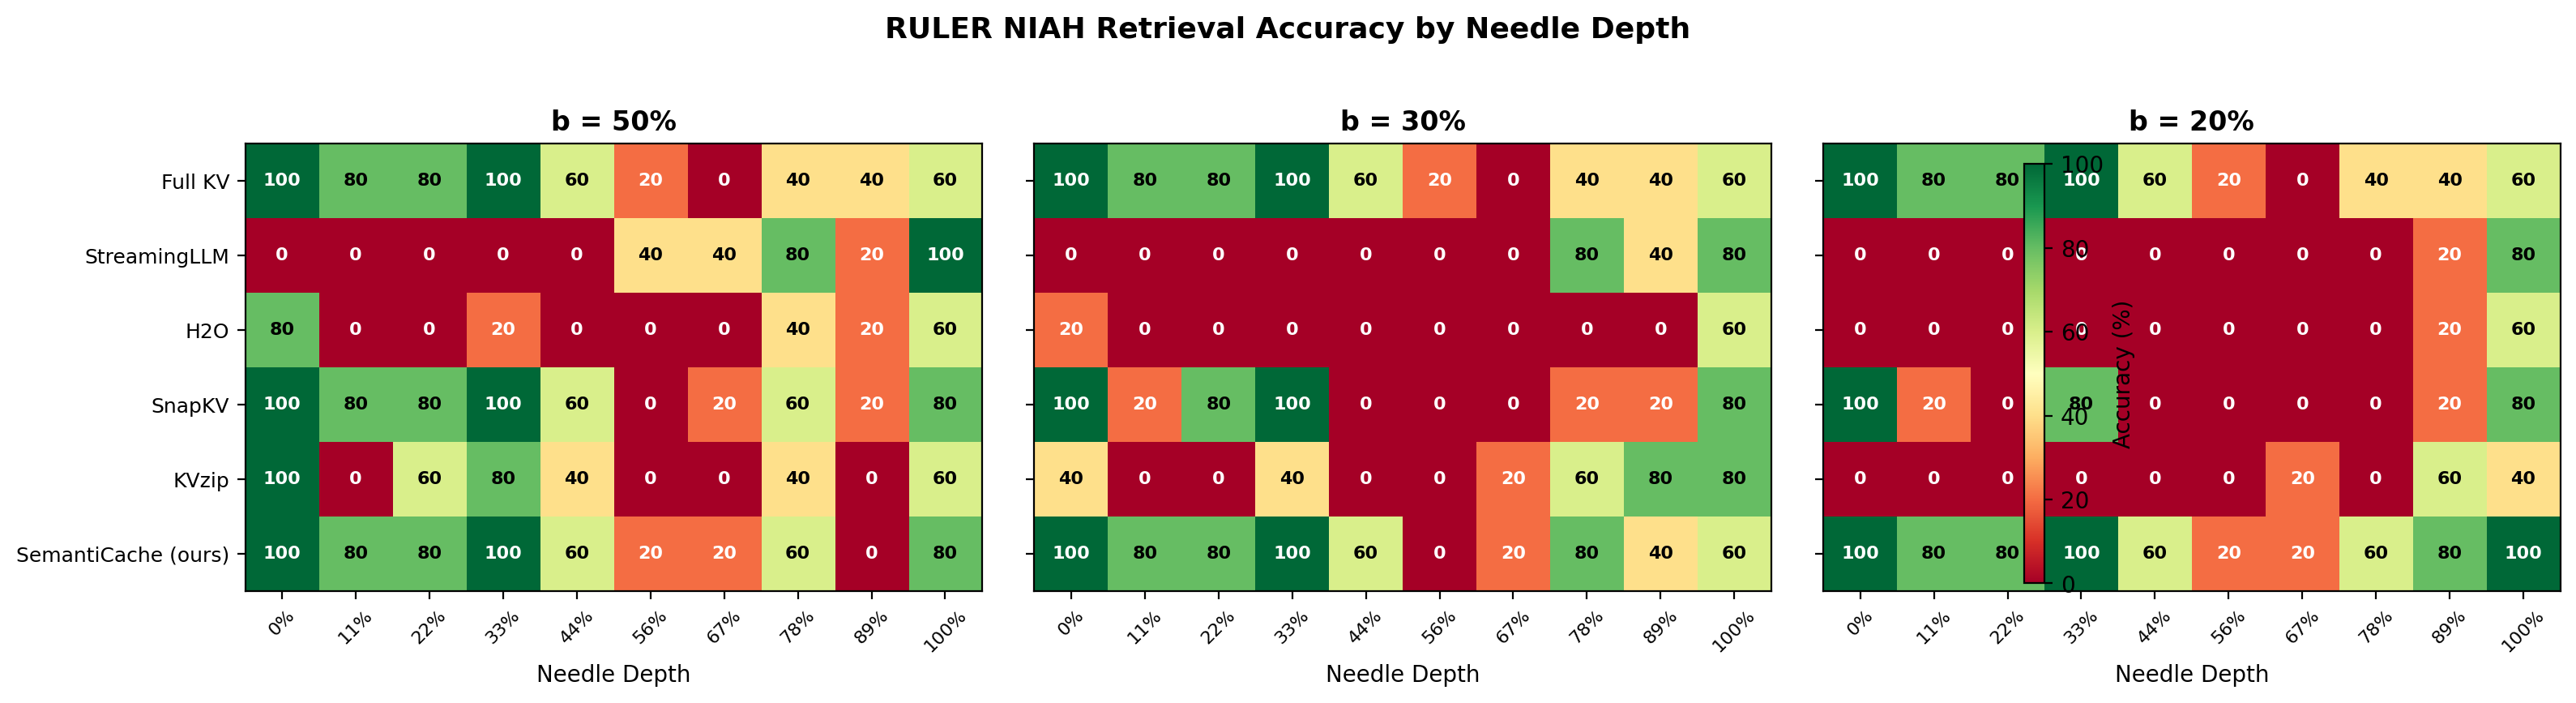
\includegraphics[width=\textwidth]{depth_heatmap.png}
\caption{Retrieval accuracy (\%) by needle depth across cache budgets.
Each cell aggregates 5 runs (5 needles at that depth).
SemantiCache is the only policy that sustains high accuracy across all depths
at $b{=}20\%$, while baselines collapse in the mid-context region.}
\label{fig:depth}
\end{figure*}

\subsection{Ablation study}

Table~\ref{tab:ablation} isolates the contribution of each signal at $b{=}20\%$.
Removing any single component causes at most a 4-point drop, suggesting the signals
are complementary rather than individually dominant.
The critical result is the bottom row: stripping \emph{all} semantic signals and
retaining only cumulative attention (the ``attention only'' variant) collapses
accuracy from 70\% to 8\%---a 62-point drop.
This confirms that the combination of information density, factual detection, and
role-aware pinning provides robust token importance estimation that no single signal
achieves alone.

\begin{table}[t]
\caption{Ablation at $b{=}20\%$. Each variant disables one component.
50 runs per variant (10 depths $\times$ 5 needles).}
\label{tab:ablation}
\centering
\begin{tabular}{lcc}
\toprule
Variant & Acc (\%) & $\Delta$ \\
\midrule
Full model (all components)                    & 70 & --- \\
\midrule
$-$ Attention ($\alpha{=}0, \gamma{=}0$)       & 70 & $\pm$0 \\
$-$ Info density ($\beta{=}0$)                  & 68 & $-$2 \\
$-$ Query relevance                             & 72 & $+$2 \\
$-$ Factual bonus                               & 66 & $-$4 \\
$-$ Role pinning                                & 68 & $-$2 \\
\midrule
Attention only (no semantic signals)            &  8 & $-$62 \\
\bottomrule
\end{tabular}
\end{table}

\subsection{Systems overhead}

Table~\ref{tab:overhead} reports per-policy latency breakdown at $b{=}20\%$,
averaged over 3 runs on the same hardware.
All eviction-based policies share an identical prefill cost (${\sim}$0.38\,s),
confirming that the overhead lies entirely in the decode phase.

KVzip incurs the highest one-time cost: its reconstruction forward pass adds
0.92\,s of snapshot latency before decoding begins, reducing throughput to
3.8\,tok/s.
SemantiCache's overhead is instead spread across decode steps: its per-step
eviction cost (8.86\,ms) is ${\sim}4{\times}$ that of attention-only policies
(H2O: 2.09\,ms) but accounts for only 3.9\% of total decode time.
SnapKV and H2O, which use simpler scoring, achieve throughput on par with
full-KV inference (7.3--7.5\,tok/s).

The tiered variant adds quantization/dequantization overhead for its warm tier
(0.13\,s quantize, 0.39\,s dequantize over 16 steps), resulting in the longest
total decode time (3.00\,s).
This cost is dominated by warm-tier materialization (1728 dequantize ops) and
represents a clear optimization target for future work.

\begin{table}[t]
\caption{Systems overhead at $b{=}20\%$ cache budget. Averaged over 3 runs
on \texttt{Qwen2.5-3B-Instruct} (4-bit NF4, 48\,GB VRAM).
Snap\,=\,one-time snapshot; Evict\,=\,mean per-step eviction latency.}
\label{tab:overhead}
\centering
\footnotesize
\setlength{\tabcolsep}{3.5pt}
\begin{tabular}{lccccc}
\toprule
Policy & Prefill & Snap & Evict/step & Decode & tok/s \\
       & (s)     & (s)  & (ms)       & (s)    &       \\
\midrule
Full KV                & 0.53 & ---   &  0.15 & 0.46 &  6.5 \\
\midrule
StreamingLLM           & 0.37 & ---   &  2.52 & 0.32 &  5.2 \\
H2O                    & 0.38 & ---   &  2.09 & 0.43 &  7.4 \\
SnapKV                 & 0.38 & 0.07  &  0.97 & 0.45 &  7.3 \\
KVzip                  & 0.38 & 0.92  &  0.96 & 1.20 &  3.8 \\
\textbf{Ours}          & 0.38 & ---   &  8.86 & 1.37 &  3.4 \\
\textbf{Ours (tiered)} & 0.38 & ---   &  7.58 & 3.00 &  4.7 \\
\bottomrule
\end{tabular}
\end{table}

%% ================================================================
\section{Discussion}
%% ================================================================

\textbf{Why does SemantiCache improve under tighter budgets?}
At generous budgets, retained tokens include both answer-critical spans and
distractors that confuse the model.
As the budget shrinks, SemantiCache's query-aware scoring concentrates retention
on factual, query-aligned tokens, effectively filtering out distractors.
The full-KV baseline, which retains \emph{all} tokens including distractors,
achieves only 58\%---demonstrating that more cache is not always better for
retrieval tasks.

\textbf{Query-aware vs.\ query-agnostic.}
KVzip (NeurIPS 2025) represents the state of the art in query-agnostic KV
compression.
Its reconstruction-based scoring identifies tokens important for reproducing the
\emph{overall} context but cannot prioritize the specific factual span needed to
answer the downstream query.
On RULER NIAH, KVzip reaches 64\% at $b{=}50\%$ but falls to 4\% at $b{=}10\%$.
This structural limitation motivates query-aware designs like SemantiCache for
retrieval-heavy workloads.

\textbf{Synergistic signals.}
The ablation shows that no single signal dominates: each contributes marginally
when removed in isolation, but removing all non-attention signals causes
catastrophic failure.
This pattern is consistent with the observation that retrieval-oriented prompts
require \emph{multiple} cues---structural, semantic, and query-specific---to
distinguish answer-bearing tokens from high-attention distractors.

\textbf{Overhead trade-off.}
Table~\ref{tab:overhead} shows that SemantiCache's per-step eviction cost
(8.86\,ms) reduces throughput to 3.4\,tok/s---roughly half the full-KV
baseline (6.5\,tok/s).
This overhead is acceptable for retrieval-heavy workloads where accuracy is
paramount, but may be significant in latency-sensitive streaming scenarios.
The tiered variant's warm-tier dequantization is the dominant bottleneck and
an immediate optimization target (e.g., GPU-side INT8 dequantize).

\textbf{Limitations.}
This study evaluates one model (\texttt{Qwen2.5-3B-Instruct}), one benchmark
(RULER NIAH), and one haystack length (${\sim}$1800 tokens).
The shared-index constraint, which retains the same token set across all layers
and heads, disadvantages methods designed for per-head selection (KVzip, SnapKV).
Extending the evaluation to longer contexts, additional benchmarks (LongBench,
NoLiMa), and larger model families remains necessary to establish generality.

%% ================================================================
\section{Related Work}
%% ================================================================

KV cache compression spans several design dimensions.
\textbf{Eviction timing}: StreamingLLM~\cite{xiao2023streamingllm} and
H2O~\cite{zhang2023h2o} evict progressively during decoding;
SnapKV~\cite{li2024snapkv} and KVzip~\cite{he2025kvzip} prune once at prefill.
\textbf{Scoring signal}: H2O uses cumulative attention; SnapKV uses
observation-window attention; KVzip uses reconstruction attention.
All are query-agnostic.
\textbf{Selection granularity}: most methods select individual tokens;
SemantiCache selects contiguous blocks.
Orthogonal approaches include quantization-based compression, which reduces
per-token storage rather than token count, and learned eviction policies that
require fine-tuning.
SemantiCache occupies a distinct point in this design space: query-aware,
multi-signal, block-level, progressive eviction without model modification.

%% ================================================================
\section{Conclusion}
%% ================================================================

SemantiCache is a query-aware KV cache eviction policy for retrieval-intensive
long-context inference.
By combining attention, information density, query relevance, factual detection,
and contiguous block retention, it achieves 70\% retrieval accuracy at 20\% cache
budget on RULER NIAH---surpassing the full-KV upper bound and outperforming the
strongest baseline by 40 points.
The method's accuracy increases as the budget shrinks, reaching 80\% at just 10\%
of the original cache.
An ablation confirms that the semantic signals act synergistically, with a 62-point
gap between the full model and the attention-only variant.
Systems profiling shows that SemantiCache's per-step eviction overhead (8.86\,ms)
accounts for under 4\% of decode time---a modest cost for a 40-point accuracy gain
over the strongest baseline.
These results demonstrate that workload-aware, multi-signal eviction is a practical
path toward memory-efficient long-context serving.

\bibliographystyle{ACM-Reference-Format}
\bibliography{systor_short_paper_refs}

\end{document}
